\documentclass[border=4pt]{standalone}
\usepackage[utf8]{inputenc}
\usepackage[T1]{fontenc}
\usepackage{amsmath,amssymb}
\usepackage[table]{xcolor}
\usepackage{tikz}
\usetikzlibrary{positioning,fit,calc,arrows.meta,shapes.geometric,decorations.pathreplacing,backgrounds}
\usepackage{pgfplots}
\pgfplotsset{compat=1.17}
\definecolor{stellantis}{RGB}{26,58,92}
\definecolor{sectionblue}{RGB}{44,95,138}
\definecolor{ddbrown}{RGB}{180,100,30}
\definecolor{ddbrownlight}{RGB}{255,243,230}
\begin{document}

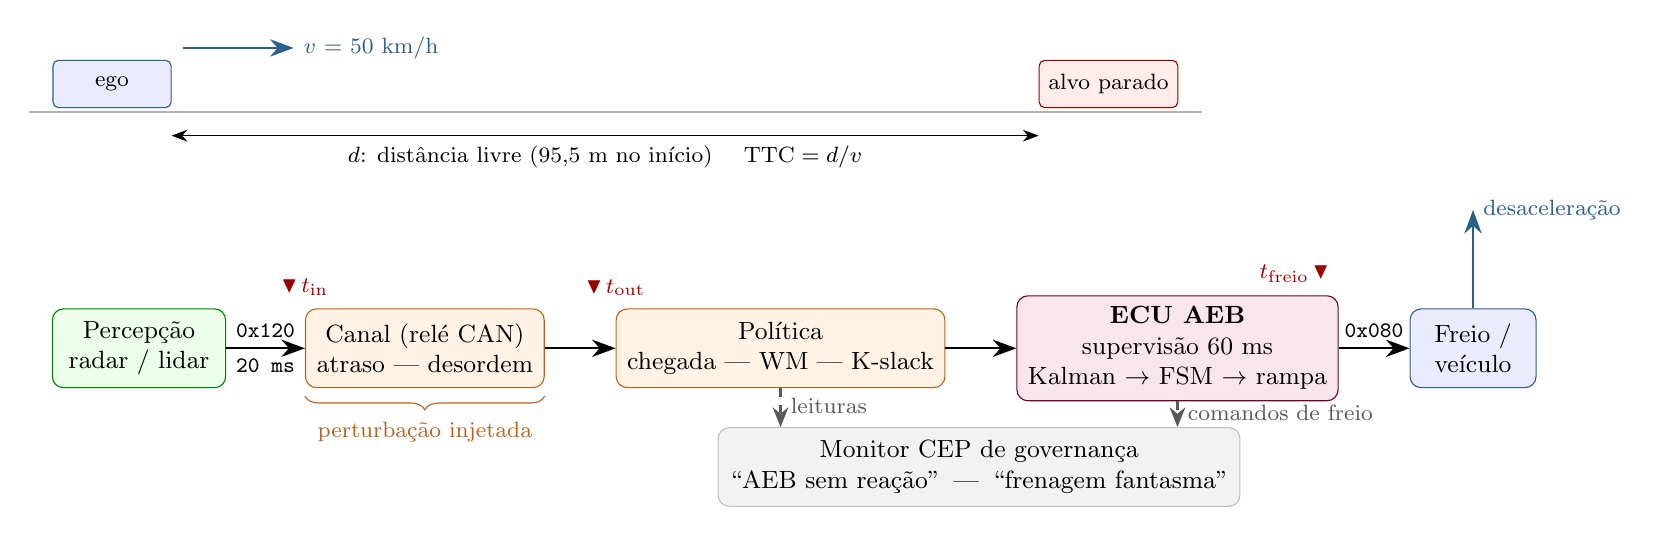
\begin{tikzpicture}[
    mod/.style={rectangle, draw, rounded corners=4pt, minimum height=1.0cm, font=\small, align=center, inner sep=4pt},
    int/.style={mod, fill=blue!8, draw=sectionblue},
    exec/.style={mod, fill=purple!10, draw=purple!60!black},
    ext/.style={mod, fill=gray!10, draw=gray!50},
    pert/.style={mod, fill=ddbrownlight, draw=ddbrown},
    ini/.style={mod, fill=green!8, draw=green!50!black},
    arr/.style={-{Stealth[length=3mm, width=2.2mm]}, thick},
    darr/.style={-{Stealth[length=2.5mm, width=2mm]}, thick, dashed, gray!70!black},
    lbl/.style={font=\footnotesize\ttfamily},
    nota/.style={font=\footnotesize, align=center},
    carro/.style={rectangle, draw, rounded corners=2pt, minimum width=1.5cm, minimum height=0.6cm, font=\footnotesize},
]
% ---- cena
\draw[gray!60, thick] (-0.3,0) -- (14.6,0);
\node[carro, fill=blue!8, draw=sectionblue, anchor=south west] (ego) at (0,0.05) {ego};
\node[carro, fill=red!8, draw=red!60!black, anchor=south east] (alvo) at (14.3,0.05) {alvo parado};
\draw[arr, sectionblue] ($(ego.north east)+(0.15,0.15)$) -- ++(1.4,0) node[right, font=\footnotesize, sectionblue] {$v$ = 50 km/h};
\draw[<->, >={Stealth[length=2mm]}] ($(ego.south east)+(0,-0.35)$) -- ($(alvo.south west)+(0,-0.35)$)
     node[midway, below, font=\footnotesize] {$d$: distância livre (95{,}5 m no início) \quad $\mathrm{TTC} = d/v$};
% ---- caminho do sinal
\begin{scope}[yshift=-3.0cm]
\node[ini, minimum width=2.2cm] (perc) at (1.1,0) {Percepção\\radar / lidar};
\node[pert, minimum width=2.4cm, right=1.0cm of perc] (canal) {Canal (relé CAN)\\atraso | desordem};
\node[pert, minimum width=2.4cm, right=0.9cm of canal] (pol) {Política\\chegada | WM | K-slack};
\node[exec, minimum width=3.0cm, right=0.9cm of pol] (ecu) {\textbf{ECU AEB}\\supervisão 60 ms\\Kalman $\to$ FSM $\to$ rampa};
\node[int, minimum width=1.6cm, right=0.9cm of ecu] (frei) {Freio /\\veículo};
\draw[arr] (perc) -- node[lbl, above] {0x120} node[lbl, below] {20 ms} (canal);
\draw[arr] (canal) -- (pol);
\draw[arr] (pol) -- (ecu);
\draw[arr] (ecu) -- node[lbl, above] {0x080} (frei);
\draw[arr, sectionblue] (frei.north) -- ++(0,1.25) node[right, nota, sectionblue] {desaceleração};
\node[ext, minimum width=5.6cm, below=1.0cm of $(pol)!0.5!(ecu)$] (mon) {Monitor CEP de governança\\``AEB sem reação'' \,|\, ``frenagem fantasma''};
\draw[darr] (pol.south) -- node[nota, right, pos=0.45] {leituras} (pol.south |- mon.north);
\draw[darr] (ecu.south) -- node[nota, right, pos=0.45] {comandos de freio} (ecu.south |- mon.north);
% marcadores de medição
\foreach \n/\l in {canal/t_{\mathrm{in}}, pol/t_{\mathrm{out}}}
  { \node[font=\footnotesize, red!60!black, above=1pt of \n.north west] {$\blacktriangledown\, \l$}; }
\node[font=\footnotesize, red!60!black, above=1pt of ecu.north east, anchor=south east] {$t_{\mathrm{freio}}\,\blacktriangledown$};
\draw[decorate, decoration={brace, amplitude=5pt, mirror}, ddbrown] ($(canal.south west)+(0,-0.1)$) -- ($(canal.south east)+(0,-0.1)$)
   node[midway, below=6pt, nota, ddbrown] {perturbação injetada};
\end{scope}
\end{tikzpicture}
\end{document}
